\documentclass{article}
\usepackage[utf8]{inputenc}

\title{Assignment 4}
\author{Benny Chen}
\date{\today}

\usepackage{color}
\usepackage{amsthm}
\usepackage{amssymb} 
\usepackage{amsmath}
\usepackage{listings}
\usepackage{xcolor}
\usepackage{listings}
\usepackage{graphicx}
\usepackage{enumitem}
\usepackage[hidelinks]{hyperref}

\definecolor{codegreen}{rgb}{0,0.6,0}
\definecolor{codegray}{rgb}{0.5,0.5,0.5}
\definecolor{codepurple}{rgb}{0.58,0,0.82}
\definecolor{backcolour}{rgb}{0.95,0.95,0.92}

\lstdefinestyle{mystyle}{
    backgroundcolor=\color{backcolour},   
    commentstyle=\color{codegreen},
    keywordstyle=\color{magenta},
    numberstyle=\tiny\color{codegray},
    stringstyle=\color{codepurple},
    basicstyle=\ttfamily\footnotesize,
    breakatwhitespace=false,         
    breaklines=true,                 
    captionpos=b,                    
    keepspaces=true,                 
    numbers=left,                    
    numbersep=5pt,                  
    showspaces=false,                
    showstringspaces=false,
    showtabs=false,                  
    tabsize=2
}

\lstset{style=mystyle}

\begin{document}

\maketitle

\section{Simple Backward Propagation}

Consider this convolutional neural network architecture.

\begin{center}
    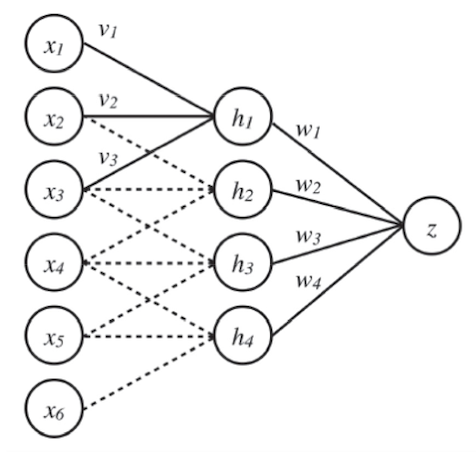
\includegraphics[scale=0.5]{images/Q1P1.png}
\end{center}

In the first layer, we have a one-dimensional convolution with a single filter of size 3 such that

\begin{equation}
    h_i = s(\sum_{j=1}^{3} v_j x_{i+j-1})
\end{equation}

The second layer is fully connected, such that

\begin{equation}
    z = \sum_{i=1}^{4} w_i h_i
\end{equation}

The hidden units' activation function (x) is the logistic (sigmoid) function with derivative

\begin{equation}
    s'(x) = s(x)(1-s(x))
\end{equation}
The output unit is linear (no activation function).
\\
We perform gradient descent on the loss function

\begin{equation}
    R = {(y - z)}^2
\end{equation}

where y is the training label for x.

\begin{enumerate}[label= (\alph*)]
    \item What is the total number of parameters in this neural network? Recall that convolutional layers share weights. There are no bias terms.
    \item Compute $\partial R / \partial w_i$. (Hint: in terms of $y, z$, and $h_i$)
    \item Compute $\partial R / \partial v_j$. (Hint: in terms of $w_i, h_i$, and $x_{i+j-1}$)
\end{enumerate}

\subsubsection*{Answer:}
\begin{enumerate}[label= (\alph*)]
    \item There are 3 parameters in the first layer and 4 parameters in the second layer. Therefore, there are 7 parameters in total.
    \item 
    \begin{equation*}
        \frac{\partial R}{\partial w_i} = -2(y-z)h_i
    \end{equation*}
    \item
    \begin{equation*}
        \frac{\partial R}{\partial v_j} = \frac{\partial R}{\partial z} \frac{\partial z}{\partial h_i} \frac{\partial h_i}{\partial v_j} = -2(y-z)\sum_{i=1}^{4}w_i h_i (1-h_i) x_{i+j-1}
    \end{equation*}
\end{enumerate}

\section{Convolution Neural Network}

Consider a convolutional neural network (CNN) for reading the handwritten MNIST letters, which are $28 \times 28$ timages. Suppose the first hidden layer is a convolutional layer with 20 different $5 \times 5$ filters, applied to the input image with a stride of 1. Each filter has a bias weight. No padding operation is applied.

\begin{enumerate}[label= (\alph*)]
    \item How many weights (parameters) does this CNN layer use?
    \item What will be the output dimension of feature map after this layer?
\end{enumerate}

\subsubsection*{Answer:}
\begin{enumerate}[label= (\alph*)]
    \item \begin{equation*}
        \text{Number of weights} = 20 \times (5 \times 5 + 1) = 520
    \end{equation*}
    \item \begin{equation*}
        \text{Output dimension} = 28 - 5 + 1 = 24
    \end{equation*}
\end{enumerate}

\section{LSTM True or False plus Explanation}

Suppose that here are the defining equations for a LSTM cell (might differ from the lecture note).

\begin{equation}
        i_t = \sigma(W^{(i)} x_t + U^{(i)} h_{t-1}) 
\end{equation}

\begin{equation}
    f_t = \sigma(W^{(f)} x_t + U^{(f)} h_{t-1}) 
\end{equation}

\begin{equation}
    o_t = \sigma(W^{(o)} x_t + U^{(o)} h_{t-1}) 
\end{equation}

\begin{equation}
    \tilde{c}_t = \tanh(W^{(c)} x_t + U^{(c)} h_{t-1}) 
\end{equation}

\begin{equation}
    c_t = f_t \circ c_{t-1} + i_t \circ \tilde{c}_t 
\end{equation}

\begin{equation}
    h_t = o_t \circ \tanh(c_t)
\end{equation}
\\
Here the symbol $\circ$ denotes element-wise multiplication and that $\sigma(\cdot)$ denotes the sigmoid function.
\\
Provide True or False for the following and briefly justify your answer
\begin{enumerate}[label= (\alph*)]
    \item If $x_t$ is the 0 vector, then $h_t = h_{t-1}$.
    \item The entries of $f_t,i_t,o_t$ are non-negative.
\end{enumerate}

\subsubsection*{Answer:}
\begin{enumerate}[label= (\alph*)]
    \item False. If $x_t$ is the 0 vector, then $i_t = f_t = o_t = 0$. Therefore, $c_t = c_{t-1}$ and $h_t = 0$
    \item True. The sigmoid function has a range of $[0, 1]$.
\end{enumerate}

\end{document}